\section{Can relationship use survive a change of world?}
\label{sec:transfer}

The transfer study asks whether relationship selection remains portable beyond
one prompt. Improvements in response format, answer marginals, or generic
campaign--poll knowledge do not require matching a particular episode's
evidence to its outcome. The transfer study isolates that match.

\subsection{Transfer under domain and mechanism shift}
\label{sec:exp3}

Training occurs only in Coin City under the direct, one-period relationship
\(x_t\rightarrow y_{t+1}\). Every prompt contains two complete reference cases, a
partially observed target, a pathway description, and a multi-outcome query. The
\emph{episode-matched} arm pairs prompt \(i\) with its own answer key. The
\emph{population-prior} control uses byte-identical prompts and the same multiset
of answer keys, but applies a fixed within-evidence-depth derangement. Thus both
arms see the same inputs and answer distribution; only the prompt--outcome
correspondence is removed from the control.

At evaluation, we change both the domain and the response mechanism. Coin City uses weekly campaign news and candidate
support; held-out Coin Harbor uses shipping bulletins and a cargo-flow index over
tide cycles. Coin Harbor is not a relabeling: it also changes the baseline and
support, driver and intervention distributions, observation noise, terminology,
units, and time scale while preserving the task template and latent response
mechanisms. Separately, a mediated, persistent mechanism replaces the direct
response.
Figure~\ref{fig:exp3-transfer-grid} defines the resulting four evaluation cells. Their
factorial combination yields in-distribution, domain-shift, mechanism-shift, and
joint-shift cells, none of which names a graph to the model. The primary
comparison is population-prior minus episode-matched response MAE in the joint
cell. Training uses three seeds per arm, and evaluation averages five stochastic
draws on 1,440 shared tasks before a paired seed-first bootstrap
(Appendix~\ref{app:exp3-complete-training-setup}).

\begingroup
\makeatletter
\def\input@path{{../}}
\makeatother
% Experiment 3 transfer results, laid out on the same 2x2 grid as the design
% figure (Figure~\ref{fig:exp3-transfer-grid}) so the reader reads results in the
% cells they were introduced in: mechanism down the rows, surface domain across
% the columns, the trained cell shaded blue and the three held-out cells green.
%
% Every number comes from tables/exp3_coin_qwen3_8b_stochastic_data.tex,
% regenerated by coin_city_structural/make_qwen3_8b_endpoint_outputs.py. Bar
% lengths share one scale
% (\cciPeak) across all four cells so cells are comparable by eye. Do not put
% formatting logic here: emphasis on an interval that excludes zero is decided
% by the generator and arrives pre-set in \cci*delta.
% generated by coin_city_structural/make_qwen3_8b_endpoint_outputs.py -- do not edit
\newcommand{\cciPeak}{7.30}
\newcommand{\cciIDbase}{3.96}
\newcommand{\cciIDprior}{0.53}
\newcommand{\cciIDmatched}{0.45}
\newcommand{\cciIDdelta}{\textbf{0.08} [0.002, 0.187]}
\newcommand{\cciDomainbase}{7.30}
\newcommand{\cciDomainprior}{2.03}
\newcommand{\cciDomainmatched}{1.79}
\newcommand{\cciDomaindelta}{\textbf{0.24} [0.03, 0.55]}
\newcommand{\cciStructurebase}{2.30}
\newcommand{\cciStructureprior}{2.36}
\newcommand{\cciStructurematched}{2.33}
\newcommand{\cciStructuredelta}{0.03 [-0.01, 0.07]}
\newcommand{\cciJointbase}{5.72}
\newcommand{\cciJointprior}{4.71}
\newcommand{\cciJointmatched}{4.46}
\newcommand{\cciJointdelta}{\textbf{0.25} [0.06, 0.47]}

\begin{figure}[!ht]
\centering
\definecolor{gCityFill}{HTML}{E8F2FB}
\definecolor{gCityEdge}{HTML}{4F7EA8}
\definecolor{gHarborEdge}{HTML}{3F8E82}
\definecolor{gTestFill}{HTML}{E7F4EA}
\definecolor{gTestEdge}{HTML}{6FA97F}
\definecolor{gTestChip}{HTML}{5E9470}
\definecolor{gCoinFill}{HTML}{FFF2CC}
\definecolor{gCoinRim}{HTML}{D6B656}
\definecolor{gInk}{HTML}{3F4550}
\definecolor{gMute}{HTML}{8A93A3}
\definecolor{gBarBase}{HTML}{C3CBD4}
\definecolor{gBarLess}{HTML}{A9B4C0}
\definecolor{gBarPrior}{HTML}{7C93AD}
\definecolor{gBarMatched}{HTML}{4F7EA8}
\newcommand{\gcoincity}[2]{%
  \begin{scope}[shift={(#1,#2)},scale=0.70]
    \fill[gCoinFill] (0,0) circle (.37);
    \draw[gCoinRim,line width=.75pt] (0,0) circle (.37);
    \fill[gCityEdge] (-.23,-.18) rectangle (-.10,.04);
    \fill[gCityEdge] (-.07,-.18) rectangle (.07,.16);
    \fill[gCityEdge] (.10,-.18) rectangle (.24,.09);
    \draw[gCityEdge,line width=.65pt] (-.27,-.19)--(.27,-.19);
  \end{scope}}
\newcommand{\gcoinharbor}[2]{%
  \begin{scope}[shift={(#1,#2)},scale=0.70]
    \fill[gCoinFill] (0,0) circle (.37);
    \draw[gCoinRim,line width=.75pt] (0,0) circle (.37);
    \fill[gHarborEdge] (-.24,-.05)--(.24,-.05)--(.15,-.18)--(-.15,-.18)--cycle;
    \draw[gHarborEdge,line width=.7pt] (-.01,-.05)--(-.01,.15)--(.15,.02)--(-.01,.02);
    \draw[gHarborEdge,line width=.55pt]
      (-.26,-.24)..controls(-.18,-.19)and(-.10,-.29)..(-.02,-.24)
      ..controls(.06,-.19)and(.14,-.29)..(.26,-.24);
  \end{scope}}
% One results card. #1 cx, #2 cy, #3 cell name, #4 chip text, #5 chip fill,
% #6..#8 base/prior/episode-matched MAE; the contrast is placed separately.
\newcommand{\gcard}[8]{%
  \node[cellname] at (#1-2.66,#2+0.78) {#3};
  \node[chip, fill=#5] at (#1+2.66,#2+0.78) {#4};
  \foreach \arm/\val/\col/\dy in {%
      base/#6/gBarBase/0.34, prior/#7/gBarPrior/0.00,
      episode-matched/#8/gBarMatched/-0.34}{%
    \node[armlab] at (#1-2.66,#2+\dy) {\arm};
    \fill[\col, rounded corners=1pt]
      (#1-0.55,#2+\dy-0.075) rectangle (#1-0.55+\val*2.55/\cciPeak,#2+\dy+0.075);
    \node[armval] at (#1-0.43+\val*2.55/\cciPeak,#2+\dy) {\val};}}
\resizebox{.96\linewidth}{!}{%
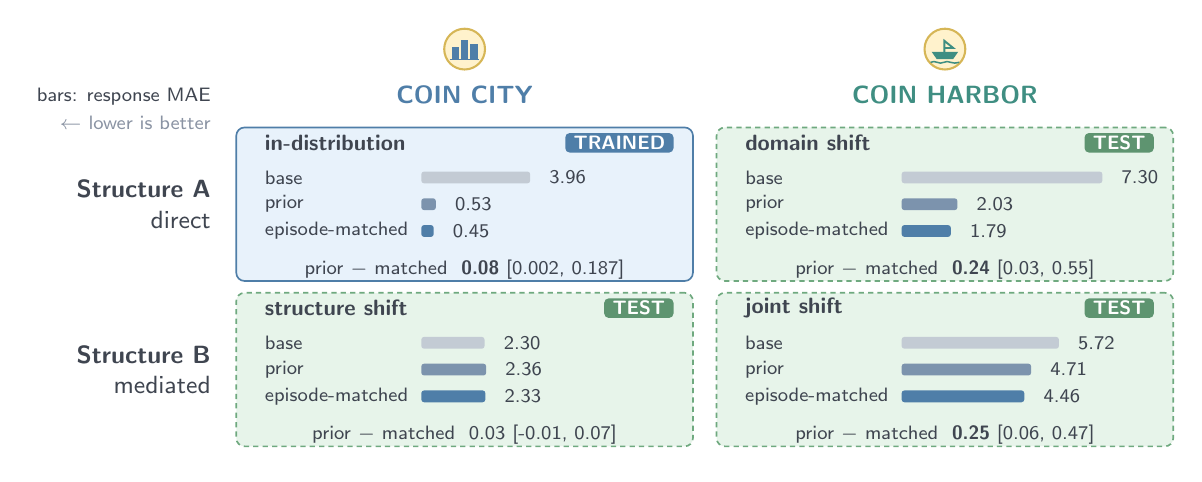
\begin{tikzpicture}[
  x=1cm, y=1cm,
  card/.style={rounded corners=3pt, minimum width=5.80cm, minimum height=1.95cm,
    line width=.6pt, inner sep=0pt},
  traincard/.style={card, draw=gCityEdge, fill=gCityFill},
  testcard/.style={card, draw=gTestEdge, fill=gTestFill,
    dash pattern=on 1.9pt off 1.5pt},
  dname/.style={anchor=south, font=\sffamily\bfseries\small},
  rname/.style={anchor=east, align=right, font=\sffamily\small, text=gInk},
  cellname/.style={anchor=west, font=\sffamily\bfseries\footnotesize, text=gInk},
  chip/.style={anchor=east, rounded corners=1.6pt, draw=none, text=white,
    inner xsep=3pt, inner ysep=1.1pt, font=\sffamily\bfseries\scriptsize},
  armlab/.style={anchor=west, font=\sffamily\scriptsize, text=gInk},
  armval/.style={anchor=west, font=\sffamily\scriptsize, text=gInk},
  delta/.style={anchor=center, font=\sffamily\scriptsize, text=gInk},
  legend/.style={anchor=east, font=\sffamily\scriptsize},
]
% ---- domain columns ------------------------------------------------------
\gcoincity{2.90}{3.22}
\gcoinharbor{9.00}{3.22}
\node[dname, text=gCityEdge]   at (2.90,2.40) {COIN CITY};
\node[dname, text=gHarborEdge] at (9.00,2.40) {COIN HARBOR};

% ---- what the bars mean, and which way is good --------------------------
\node[legend, text=gInk]  at (-0.20,2.62) {bars: response MAE};
\node[legend, text=gMute] at (-0.20,2.28) {$\leftarrow$ lower is better};

% ---- mechanism rows ------------------------------------------------------
\node[rname] at (-0.20,1.25) {\textbf{Structure A}\\ direct};
\node[rname] at (-0.20,-0.85) {\textbf{Structure B}\\ mediated};

% ---- the four result cards ----------------------------------------------
\node[traincard] at (2.90,1.25) {};
\node[testcard]  at (9.00,1.25) {};
\node[testcard]  at (2.90,-0.85) {};
\node[testcard]  at (9.00,-0.85) {};

\gcard{2.90}{1.25}{in-distribution}{TRAINED}{gCityEdge}
  {\cciIDbase}{\cciIDprior}{\cciIDmatched}
\node[delta] at (2.90,0.42) {prior $-$ matched\ \ \cciIDdelta};

\gcard{9.00}{1.25}{domain shift}{TEST}{gTestChip}
  {\cciDomainbase}{\cciDomainprior}{\cciDomainmatched}
\node[delta] at (9.00,0.42) {prior $-$ matched\ \ \cciDomaindelta};

\gcard{2.90}{-0.85}{structure shift}{TEST}{gTestChip}
  {\cciStructurebase}{\cciStructureprior}{\cciStructurematched}
\node[delta] at (2.90,-1.68) {prior $-$ matched\ \ \cciStructuredelta};

\gcard{9.00}{-0.85}{joint shift}{TEST}{gTestChip}
  {\cciJointbase}{\cciJointprior}{\cciJointmatched}
\node[delta] at (9.00,-1.68) {prior $-$ matched\ \ \cciJointdelta};
\end{tikzpicture}%
}
\caption{\textbf{Qwen3-8B Coin City transfer at round 300 under five-draw
stochastic decoding.} Bars show task-averaged response MAE over four evidence
depths; trained arms average three seeds. Each cell prints the paired seed-first
prior-minus-matched contrast, bold when its 95\% interval excludes zero.}
\label{fig:exp3-transfer-results}
\end{figure}

\endgroup

\paragraph{Finding: episode matching adds a transfer gain.}
Figure~\ref{fig:exp3-transfer-results} reports the four-cell comparison. For
Qwen3-8B under joint shift, response MAE is \(5.72\) for the untrained base,
\(4.71\) after population-prior training, and \(4.46\) after episode-matched
training. The matched advantage over the distribution control is
\(.251\,[.058,.470]\). It has the lower point estimate in all four cells.
Qwen3-4B replicates the joint-cell contrast. Removing or reversing the pathway description also degrades the matched
model. Transferred forecasts therefore remain responsive to relational language.

The control also isolates the gain from episode matching. Episode matching
accounts for about one fifth of Qwen3-8B's total improvement over base in the
joint cell, beyond shared format and population learning. The replicated
joint-shift contrast shows that matching each episode's evidence to its outcome
adds transfer value across the two tested model scales.

\subsection{External grounding: held-out historical markets}
\label{sec:exp4}

\begin{figure}[!t]
\centering

\includegraphics[width=\linewidth]{exp4_qwen_scale_results.pdf}
\caption{\textbf{Outcome-based training improves the tested bases, and several
trained checkpoints reach the crowd-level floor.} Performance is nonmonotonic
across the tested Qwen sizes. The left panel connects checkpoints only within the
Qwen and Llama families; small points are training seeds. Hosted deployments in the right panel are categorical references.
Panels use different Brier scales.}
\label{fig:sealed-market-grounding}
\end{figure}

A separate historical-market study tests outcome-based training on real,
held-out events. Resolved political, governmental, macroeconomic, and geopolitical markets
are censored before resolution. Prompts contain only the question, rules, cutoff,
and genuine pre-cutoff prices; outcomes and post-cutoff fields are withheld.
Calendar splits prevent event and normalized question families from crossing
training, development, and test. Qwen3 and Llama checkpoints receive rank-32 LoRA
training with reward \(1-(\hat p-y)^2\), the complement of Brier loss. A
318-market holdout is disjoint from training, development, and the earlier
1,024-market test, and every endpoint is evaluated with five stochastic draws
(Appendix~\ref{app:exp3b-protocol}).

Figure~\ref{fig:sealed-market-grounding} separates the local scaling comparison
from hosted reference systems. Proper-score training lowers mean Brier relative
to every tested base checkpoint.
The trained Qwen series is nonmonotonic from 1.7B to 14B. Across both
evaluated families, Qwen3-1.7B, Qwen3-14B, and Llama-3.1-8B reach a practical
floor set by contemporaneous Polymarket forecasts: each trained-minus-market
interval crosses zero. Hosted systems are categorical reference points, not members of
the local scaling curve.

The controlled factorial separates episode-level relationship learning from
shared format and answer-distribution gains. The historical study measures
training effects on held-out real events. Relationship use and external accuracy
are separate claims.
